\section{IoT}



\textit{Internet of Things (IoT)} adalah sebuah infrastruktur dari objek, orang, sistem, serta sumber daya informasi yang saling terhubung dengan layanan cerdas untuk memproses informasi dari dunia fisik dan virtual \parencite{Dias2019}. Konsep dan paradigma \textit{Internet of Things} ini merupakan perwujudan dari evolusi teknologi informasi karena dapat membuat kehidupan menjadi lebih baik dalam berbagai sektor. Setiap objek yang ditemukan pada kegiatan sehari-hari, bertransformasi menjadi entitas cerdas yang mampu berinteraksi dengan lingkungan sekitarnya dan jaringan digital secara lebih luas. IoT memperkenalkan kemungkinan baru dalam otomatisasi dan pengambilan keputusan yang berbasis data, membuka jalan bagi inovasi lintas sektor \parencite{madakam2015internet}.

\begin{figure}[ht]
  \centering
  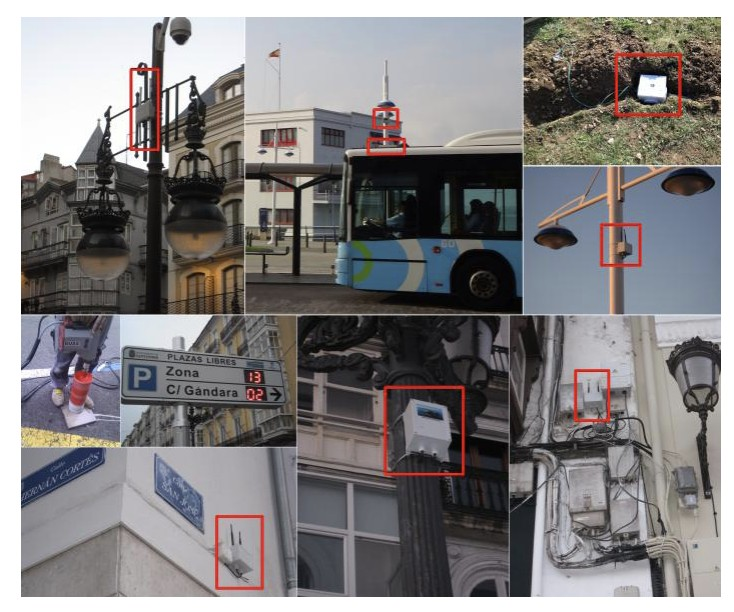
\includegraphics[width=0.8\textwidth]{resources/chapter-2/gambar-iot.jpg}
  \caption{Perangkat IoT yang Terdapat pada Lingkungan Sekitar \parencite{sotres2017practical}}
  \label{fig:iot-kehidupan-sehari-hari}
\end{figure}

IoT memiliki aplikasi yang luas di berbagai sektor, termasuk industri, kesehatan, transportasi, dan pertanian. Dalam sektor industri, IoT memungkinkan otomatisasi proses dan pemantauan efisiensi mesin secara real-time. Di bidang kesehatan, IoT berkontribusi pada pengembangan perangkat medis yang terhubung untuk pemantauan kesehatan pasien. Dalam transportasi, IoT mendukung pengembangan kendaraan otonom dan sistem manajemen lalu lintas cerdas. Di sektor pertanian, IoT digunakan untuk memantau kondisi tanah dan iklim, membantu petani dalam pengambilan keputusan seperti pada gambar \ref{fig:iot-kehidupan-sehari-hari}

, IoT dapat dibagi menjadi tiga lapisan, yaitu lapisan persepsi, lapisan jaringan, dan lapisan aplikasi secara berurutan. Lapisan persepsi bertanggung jawab atas pengumpulan data dalam IoT. Lapisan ini terdiri dari berbagai jenis sensor, seperti sensor suhu, sensor kelembaban, RFID, kamera, GPS, dan sebagainya. Lapisan jaringan terdiri dari berbagai jenis jaringan, seperti internet, jaringan komunikasi 2G dan 3G, serta jaringan siaran. Lapisan jaringan terutama digunakan untuk mengumpulkan data dari lapisan persepsi dan memproses data tersebut untuk lapisan aplikasi. Lapisan terakhir, yaitu lapisan aplikasi, adalah antarmuka antara pengguna dan IoT. Banyak aplikasi, termasuk logistik, rantai pasokan, pertanian, industri, keamanan publik, pengelolaan perkotaan, telemedis, rumah pintar, transportasi pintar, dan pemantauan lingkungan, diaktifkan melalui IoT \parencite{SmartHomeSystemBasedOnIoTTechnologies}.

Seiring dengan bertambahnya jumlah perangkat IoT, perlu dibuat suatu cara agar sistem \textit{scalable}. \textit{Device discovery} merupakan salah satu masalah yang perlu diatasi untuk membuat sistem IoT yang \textit{scalable}. Dengan adanya \textit{device discovery}, \textit{quality of service} dapat ditingkatkan \parencite{DeviceDiscovery}. Tidak hanya itu, kemunculan berbagai perangkat IoT baru yang memerlukan \textit{update} secara berkala juga menimbulkan masalah baru yakni sulitnya melakukan \textit{update} untuk setiap perangkat yang ada apabila jumlahnya semakin meningkat sehingga peran \textit{remote deployment} menjadi sangat penting dalam menyelesaikan masalah ini \parencite{RemoteDeployment}.